\documentclass[12pt]{article}


% Overall formatting
\sloppy
\let\cleardoublepage\clearpage % do not force chapters to start on odd pages


% Graphics
\usepackage{graphicx}
\DeclareGraphicsExtensions{.png,.pdf,.jpg}
\graphicspath{{Figures/}}


\usepackage[a4paper, total={16cm,25cm}]{geometry}



% Tables
\newlength{\mytabskip}   
\setlength{\mytabskip}{-1.5ex}
\newcommand{\tabrule}{\rule[\mytabskip]{0ex}{0ex}}
\usepackage{tabularx}
%\usepackage{longtable}


% bibliography stuff 
\usepackage{natbib}
\bibliographystyle{kluwer} 


\newcommand{\unit}[1]{\ensuremath{\mathrm{#1}}}
\newcommand{\degree}{\ensuremath{\mathrm{^\circ}}}

%\newcommand{\FIXME}[1]{{\sffamily \bfseries #1}}
\newcommand{\FIXME}[1]{{\sffamily {\bfseries \textcolor{red}{FIXME:} #1}}}


\hyphenation{EUMETSAT}
\hyphenation{Metop}



\begin{document}



\noindent
\textbf{\Large Study to support the definition of Arctic Weather \vspace{1mm}\\
Satellite (AWS) high frequency channels} \vspace{8mm}\\
{\bf Patrick Eriksson, Simon Pfreundschuh and Inderpreet Kaur}\\
Department of Space, Earth and Environment\\
Chalmers University of Technology\\
SE-412\,96, Gothenburg, Sweden \vspace{10mm}

\section{Introduction}
%
\dots


\section{Data and methods}

\subsection{Atmospheric scenarios}

\subsubsection{Fascod}
\label{sec:fascod}
%
The Fascod dataset \citep{anderson1986afgl} was used to represent different
climate zones in overview calculations. The dataset consists of profiles of
pressure, temperature and volume mixing ratio profiles of various atmospheric
gases. Five climatoligies were used: tropical (TRO), mid-latitude summer (MLS),
mid-latitude winter (MLW), sub-arctic summer (SAS), and sub-arctic winter
(SAW). No hydrometeors were included in simulations involving Fascod.


\subsubsection{Bulk profile database}
%
A database of atmospheric cases was created based on data from CloudSat and
ERA-Interim. The core idea of the approach is to use CloudSat reflectivities to
obtain as realistic vertical profiles of ice hydrometeors and rain as
possible. No external CloudSat retrievals are involved. Instead the CloudSat
reflectivites are mapped to properties for the passive simulations by assuming
a particle size distribution (PSD) and a particle habit, together denoted as
the particle model. The process involves an inversion of the radar data, but as
the same particle model is used for that inversion and to map ice water content
(IWC) and rain water content (RWC) to single scattering data when performing
the passive radiative transfer calculations, the impact of clouds on the
simulated AWS data is as realistic as possible. The thin clouds not detected by
CloudSat should not be of relevance for passive measurements frequencies
350\,GHz. Background data (temperature, humidity, 10\,m wind speed, \dots) were
taken from ERA-Interim, for the time and location of the CloudSat data. Liquid
water content (LWC) was taken from ERA-Interim, as CloudSat has no sensitivity
to the hydrometeor category.

This approach for generating atmospheric scenarios has been used by us since
\citet{rydberg:nonga:09}, and more recently in e.g.\
\citet{eriksson:towar:20,barlakas:three:20}. It is also used in
\citet{ekelund:using:20}, where the approach is described more in detail. In
the cited articles, the sensor's footprint has been considered in varying
degree, as ``beam filling'' must be considered at high impact of hydrometeors.
As clear-sky and weak cloud interference are in focus in this study, and to
save calculation time, instead CloudSat data were averaged over 10\,km to form
the atmospheric cases and standard 1D radiative transfer calculations are
applied on each case (instead of applying an independent beam approximation
inside a 2D or 3D atmosphere as done in cited works).

[* Do we show comparison to ATMS, or do we refer to articles for ``validation''? ]
[* Add time and latitude ranges used * ]


\subsection{Radiative transfer simulations}
%
\subsubsection{ARTS}
%
All radiative transfer calculations are made by the Atmospheric Radiative
Transfer System (ARTS, \citet{eriksson:arts2:11,buehler:artst:18}), version
arts-2.3.????. Models and input used for absorption and hydrometeor properties
are described below. Ocean/water and land emissivities are taken from
TESSEM \citet{prigent2017sea} and TELSEM \citet{aires2011tool}, respectively.

The calculations were performed for each atmospheric cases. One ''clear-sky''
where all hydrometeors contents were set to zero, and one ``all-sky'' where IWC
and RWC derived from CloudSat reflectivities and LWC from ERA-Interim were
included. Both sets of calculations were were made by ARTS's interface to the
RT4 solver \citep{evans1995microwavec}. This ``scattering solver'' was used
also for clear-sky, to avoid a possible bias between clear-sky and all-sky for
insignificant hydrometeor contents. RT4 handles the first two elements of the
Stokes vector, that were converted to brightness temperatures for H- and V-
polarisation.


\subsubsection{Absorption models}
%
The absorption of nitrogen is modelled following \citet{pwr:93}. Nitrogen has a
significant impact at least around 325\,GHz at dry conditions. Also oxygen
absorption follows \citet{pwr:93}. Oxygen is in this study mainly of concern
for the 89\,GHz CloudSat simulations. LWC was treated to be
purely absorbing, based on \citet{ellison2007permittivity}.

For water vapour the present settings in RTTOV are applied. That is, largely
MPM89 \citep{liebe:89} is followed, but some parameters for the 22 and 183\,GHz
transitions are replaced \citep{saunders2018update,turner2019amsutran}. A basic
comparison to RTTOV (12.?) was made (with MHS as assumed sensor) and an
agreement around or better than 0.?\,K was found.


\subsubsection{Hydrometeor properties}
%
[* Write later, Simon? TRO only! *]


\subsection{Sensor characteristics}
%
The AWS satellite was assumed to be at an altitude of 600\,km. Data were
generated for sensor viewing angles (the angle from nadir) from 0$^\circ$ to
45$^\circ$, in steps of 5$^\circ$.

AWS channels that were included, and considered as fixed in terms of positions
and widths, are found in Table\dots [* Finish after talking to Anders at
Omnisys. * ]

[* Clarify what polarisation we assume for the different channels *]

[* Inderpreet: Add equation and text about polarisation rotation (ie equations
in the Sow) *]

[* Describe settings for ATMS together with results, if included *)


\section{Results}

\subsection{Overview of the 183, 229 and 325\,GHz bands}
%
The simulations in this sction are based on five Fascod climate scenarios
(Sec.~\ref{sec:fascod}), and performed with a fixed sensor viewing angle of
25$^\circ$. No hydrometeors are included. For simpler interpretetation of the
results, the reflectivity is set to have no frequency variation, i.e.\ the same
value is applied for all bands. The reflective is varied between 0 and 0.5.


\subsubsection{Clear-sky brightness temperatures}
%
Figure~\ref{fig:tb:r00} shows brightness temperatures over the three bands, for
a reflectivity of 0 (i.e.\ a blackbody surface). The figure takes into account
that the 183\,GHz channels of AWS are of single-sideband character, while for
229 and 325\,GHz averages of upper and lower sidebands are shown, plotted as
a function from the centre frequency on the lower side.

\begin{figure}[p]
  \centering
  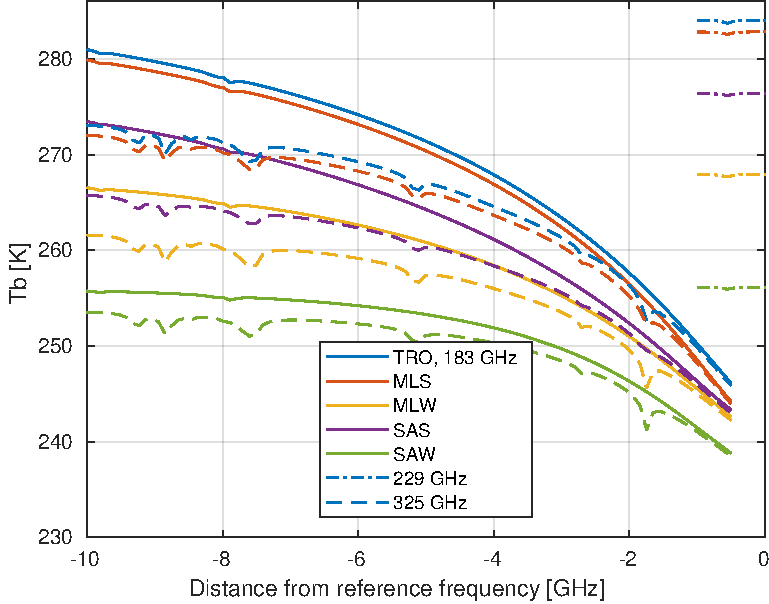
\includegraphics[width=0.75\textwidth]{fascod_tb_r000}
  \caption{Solid lines show brightness temperatures for the lower wing of the
    183.31\,GHz transition. Dashed lines represent double-sideband measurements
    around 325.15\,GHz, with the mean of upper and lower band shown on the low
    side. Dash-dotted lines represent double-sideband measurements around
    229.00\,GHz in the same manner, but only over the bandwidth of the
    potential channel. For all three bands, spectra for all five
    Fascod scenarios are included.}
  \label{fig:tb:r00}
\end{figure}
\begin{figure}[p]
  \centering
  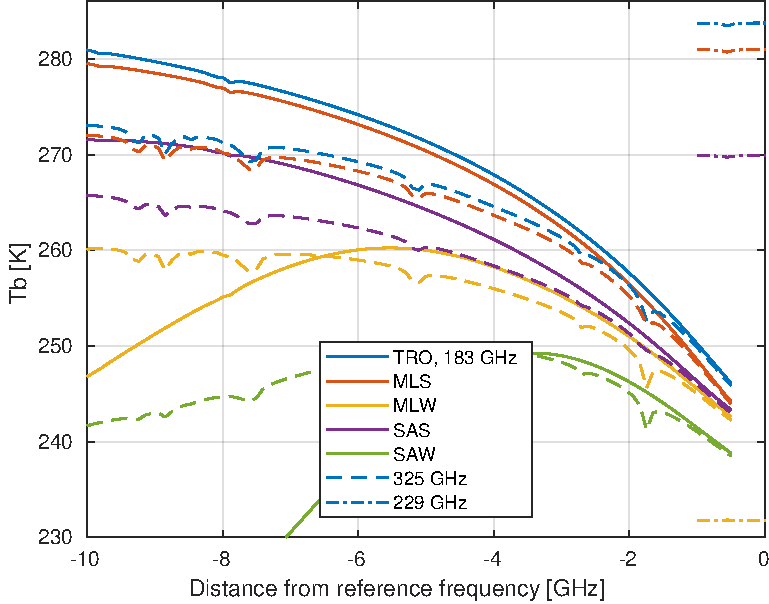
\includegraphics[width=0.75\textwidth]{fascod_tb_r050}
  \caption{Same as figure above, but with a surface reflectivity of 0.5.}
  \label{fig:tb:r00}
\end{figure}

For 183 and 325\,GHz the brightness temperatures increase when moving away from
the centre frequency of the transition. The ``kinks'' in the spectra correspond
to ozone transitions, that are both more frequent and stronger in the 325\,GHz
range than in the 183\,GHz one. See Fig.~1 of \citet{eriksson:towar:20} for how
the ozone transitions are distribbuted between the lower and uper 325\,GHz sideband. 
The spectra of 183 and 325\,GHz deviate little close to the trasition
frequency, showing that the two frequencies are of similar strength, though the
325\,GHz one is slightly weaker. The higher deviation further out in the wings
is due to different contribution of far wing and continuum absorption. This
contribution is higher at 325\,GHz. The 229\,GHz brightness temperatures is
higher than any value around 183 and 325\,GHz, as expected 229\,GHz being a
window channel.  

In Figure~\ref{fig:tb:r00} the surface reflectivity is changed to 0.5, which
should roughly correspond to the highest reflectivity encountered at these
frequencies. The differences between the two figures are small for 183 and
325\,GHz tor the tropical and the two summer scenarios. On the other hand,
there is a clear impact in the wing part of 183\,GHz for the two winter
scenarios. The same is true for 340\,GHz, but the influence of the surface
reflectivity is considerably lower. [* Comment somewhere on the implications of
this for retrievals at high latitudes *] Beside for the tropical case, for
229\,GHz there is a pronounced dependendency of the surface reflectivity, e.g.\
about 35\,K for mid-latitude winter.


\subsubsection{Clear-sky relative humidity weighting functions}
%
\dots


\subsubsection{Clear-sky transmissivities to space}
%
\dots

\bibliography{j_abbr,references}

\end{document}
